\documentclass{article}
\usepackage[utf8]{inputenc}
\usepackage{graphicx}
 
\begin{document}
\maketitle{ E-ticket}
\begin{center}

\author{Group D\\
We Works\\ \textbf{E-Ticket By Bus}\\ Group Members(4)-\\Name: Md Eyamin Molla \\ ID-19202103209(44)\\ Name: Md Rakibur Rahman Zihad\\ ID: 19201103082(43)\\ Name: Md Mohibbullah\\Id:19201103101\\ Name: Nahian Islam\\ID : 19201103028\\ Name: Raihan Ahmed\\ ID:19202103480
}
  
\newpage
\title{\huge E-Ticket by Bus\\
}
\end{center}
\begin{center}
    \section \huge \textbf{Abstract}
\end{center}
Bus e-ticket system is a web based application that works within a network. Presents a review on e-ticket system used in a bus transport system, a facility used for reserving, canceling reservations and securing reservations quickly for various types of route search. Traditional database, ticket booking and OBTRS was developed to computerize buses and. It maintains all customer details, bus details, and reservation details. To achieve the design, Imo Transport Company was chosen because of its strategic importance in Imo State. Structured Systems Analysis and Design Methodology was adopted. In addition, PHP hypertext preprocessor language was used for the front end of the software and the back end was designed using MySQL. As a result, the software is capable of improving the customer's hand and relationship management in ITC operations. Despite the current functionality of the designed software, additional functionality such as customer Use of e-mail to send tickets and notifications and cashback Ash should be implemented in the online payment system. Hence, other activities carried out by ITC should be integrated to improve the bus e-ticketing system.
\newpage
\tableofcontents
\newpage
\begin{center}
\huge \textbf{Chapter 01}
\end{center}
\subsection{Introduction}
The public bus transport system is mostly used by people in different areas like villages, and urban and metro sites. From students to many professionals are using bus transportation to reach their destinations on time. As there are multiple routes across the city, it can take just the right amount of time. Due to the demand of bus transport among the public, many facilities are being provided for the comfortable travel of all types of passengers. Although the luxury sector has improved, the ticketing system still requires cash to buy bus e-tickets. Since online bus e-ticket booking is only used for long-distance travel, city buses still suffer from the problem of cash payments. There will usually be fights, arguments and problems between bus conductors and passengers over not getting the right amount of money back. Those problems still happen to passengers on every bus every day. Therefore, online system will be introduced to facilitate currency exchange and transactions in public bus transport to solve this problem. At present, electronic ticketing machines are used to collect money in buses. In this way the rent is taken digitally with the help of smart card without money transaction. The passenger will be issued a smart card each card will have a unique ID number to store the information in the database. Govt bus tickets are available without direct payment. The amount will be deducted from each passenger's account and the account can be recharged whenever required. Each card will be provided with personal profile data, so they can calculate their statistics such as income, expenditure and transaction details like bus travel per month. The database in the transport corporation will give information like the number of passengers using a bus per day. And on a trip, areas with high crowds and times etc. So they can use that information to improve e-ticketing by hiring more buses during peak hours. In case of account the amount will be transferred to the account. So there is no need to get cash tickets from every bus conductor.
\newpage
\subsection{Problem Statement}
The system currently being used by the staff at the ticket counter is an internal system and is only used to sell bus tickets at the ticket counter. The customer has to go to the counter to buy the bus ticket or check the bus schedule. Passengers have to pay cash while buying bus tickets and sometimes they have to stand in long queues to get bus tickets which wastes a lot of time. Besides, passenger mobiles are not allowed to buy bus tickets and bus company mobiles always have busy lines.
  So online e-ticket booking will be “e-ticketing can play a great step for Bangladesh to avoid this offline problem and make great use of technology.
While working on improvements in this e-ticketing project I have identified some issues which will play an important role in the improvement of the whole project. Some problems with this project may be:\\\\
\textbullet Lack of good knowledge about software\\
\textbullet Information source\\
\textbullet Server security and maintenance\\
\textbullet Creation of eligibility database system along with information as per e-ticket booking.\\
The main problem I found is creating a simple ticket booking system to allow the user of the country because most of people don't know about the online process and can't falsify the data. Even though the system can process applications with the basic criteria and skills of Bangladeshi online users, the problem can be overcome with e-tickets.

\newpage

\subsection{Project Scope}

The E-ticket system is a web-based application. Users will have access to buses and seats on specific routes by logging in as customers. Passengers or staff will access the system by logging in through the portal where they can access all bus facilities and monitor other issues.
The main problem we found is creating a simple ticket booking system to allow the user of the country because most people don't know about the online process and can't falsify the data. Even though the system can process applications with the basic criteria and skills of Bangladesh online users, the problem can be overcome with an e-ticker.
\begin{figure}[h]
    \centering
    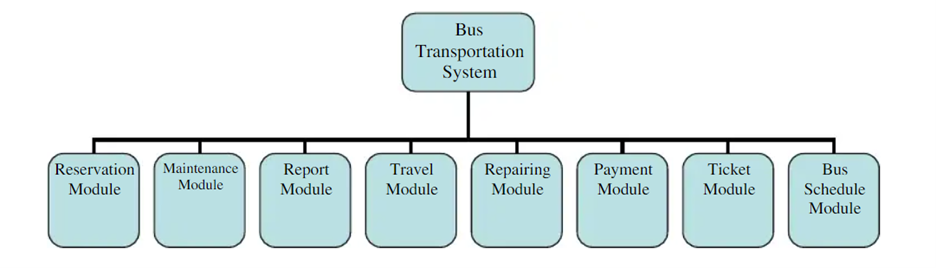
\includegraphics[width=10cm,height=6cm]{img/Picture1.png}
    \caption{Diagram}
    \label{fig:my_label}
\end{figure}

\subsection{Reservation Module}
This reservation allows passengers to book bus tickets through e-ticket online when they want to travel from one destination to another. After reserving the bus ticket the passenger must pay for the reservation online then the information will be stored in the database.
\subsection{Maintenance Module}
This module is to help maintain passenger and bus information. It is used to record passenger and staff information such as name, IC, and address and to record bus information. The purpose of using this module is to store passenger, staff, and bus information. This module has the functionality to add employee and passenger information. Then, when users need to change the information in the record, this module plays an important role to allow the user to edit and update their new information. This module helps to view employee records. Apart from that, the module helps users to delete records from a database. This maintenance module can allow the user to add new bus information when the company buys a new bus. It can change, view or delete bus information. The maintenance system allows the user to view the maintenance of the bus service to remind the user that the bus is always being maintained or checked. This maintenance module can allow staff to upload photos of passengers to understand what staff and passengers look like. When buses go for maintenance staff can upload pictures of buses so they know which bus is being maintained and when.
\subsection{Repairing Module}
This module allows adding new service information to the e-ticket database when the bus is sent for service so that the administrator chooses which service company to send the bus for service. After returning the bus from the service company, the admin can edit the service details like inserting the maintenance fee for the particular bus. Admin can view service details to know which bus is still under maintenance so they can arrange schedules according to bus number and bus status.
\subsection{Bus Scheduling Module}
This bus scheduling module is used by the administrator to add new schedules and own destinations for the driver to run the bus as per the schedule. Admin is used to deleting and add new driver information and schedule details. Drivers can also see what time they are doing, so they can use it to see if the schedule is right to get from one destination to another on time.
\newpage
\begin{center}
\section  \huge \textbf{Chapter 02}    
\end{center}
\subsection{Literature Review}

    
     An online ticket booking system is the most used technology by common people in developed countries and now developing countries are starting to use this technology. Day by day this process is getting easier than before and all classes of people will one day be familiar with this technology. The basic concept of the e-ticket management system is to allow users to find travel information, fares, availability, etc. In past e-ticket or online booking system was not so popular and people used to book tickets manually through the e-ticket office. Eventually, these were replaced by complex computerized reservation systems. Initially, e-ticketing was extended for use by agents who could query the systems and make reservations themselves. If a passenger wants to book a seat or wants to go within a schedule then he can do the booking online mode. Hence there was a need for a web-based booking system that allows passengers to directly retrieve information about schedules, bookings etc. This was the first introduction of an internet booking engine. The overall overview of this ticket booking system is, it will work for any user by visiting the webpage online. Then anyone wishing to book a ticket online can register for an online account with an email address and password as login criteria. Users will be able to view the availability of specific and desired tickets and proceed with the confirmation. There will be an online account directly linked to the database server that allows users to view, cancel or modify tickets by correcting their personal details as well as paying certain fines or surcharges. The most important feature is online payment, which allows people to pay online through bank cards and secure transactions. As mentioned earlier, online ticket booking systems are no longer a surprise for developed countries. A lot of work has been done in the past to improve the online reservation system and more work is going on. This entire project work is not a new method or concept but a shadow of the previous work, rather a new way and a step in development for a developing region like Bangladesh. Users of this online e-ticket management system can definitely get the most out of it.
However, the entire research method was to the best of my knowledge and programming skills. Future work is required to develop an online e-ticket management system Although, the implementation of the system is related to the work of the past, still this method needs more time to become familiar and implemented in a wide range of processes. User comfort capabilities and online security have a lot of work to do in the future. Future improvements can be made gradually over the coming years.
More about this source text is required for additional translation information
Send feedback\\
Side Online ticket booking System at a glance:-
\begin{itemize}
    \item Viewers can view or visit the web page
    \item Then it match user desired seat with the database and shows whether user’s desired seat is available or not.
    \item In this system first of all the system match the user who want to log into the system with the registered user.
    \item Next it matches the user bank account with the bank account whether the account number is valid and has enough money to buy the ticket.
    \item And again a user can cancel his ticket using the system
\end{itemize}

\subsection{Previous related works}
With the rise of modern science and technology, online ticket booking system is fast no longer a wonder for the countries of the world. All countries feel the need for convenient customer service and efficient ticket management when e-ticketing systems are first launched. Gradually, ticket booking systems have managed more platforms and security measures to keep up with the modern computerization race. My country is far behind other countries in implementing our e-ticket management system and online booking system. Many previous applications, designs and studies have been taken into consideration while developing the e-ticket system for Bangladesh. Use of old traditional process but I try to make the total process of ticket booking process simple and user friendly. Bangladesh has adopted similar measures for e-ticket booking in recent years. However, the work and process are not widely used in Bangladesh due to public awareness, internet usage trend, financial capability and ignorance.
\newpage
\begin{center}
    \section \huge \textbf{Chapter 03}
\end{center}
\subsection{Methodology}
It is important to fulfill the planning of the implementation phase. This can only be done if the proper methodology is selected. The methodology is important to make sure all project life cycle activities are being carried out without any shortcuts. The methodology helps the system developers to take one step at a time towards accomplishing the full system. The following section discusses the choice of methodology for the implementation of the Online Bus Ticketing System for Modern Coast Bus Company.
\begin{figure}[h]
    \centering
    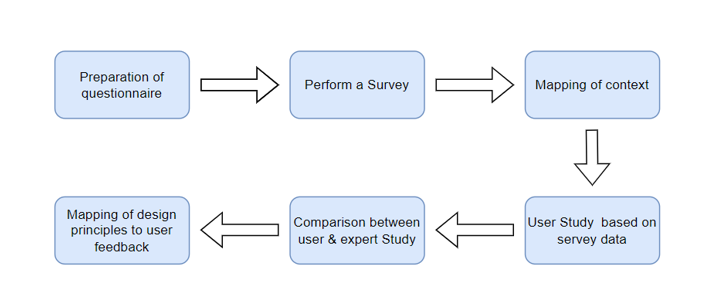
\includegraphics[width=10cm, height=6cm]{img/methelodo.png}
    \caption{Context mapping theme}
    \label{fig:my_label}
\end{figure}
\subsection{System development methodology }
The e-ticketing system has gone through all stages of the development life cycle. A waterfall approach was used to develop this e-ticketing system. This method included the following steps: feasibility study, requirements analysis, and coding, testing, and integration. Each step required a different amount of effort and each step had a specific start and point. Each phase must be completed before starting the next phase:
\begin{figure}[h]
    \centering
    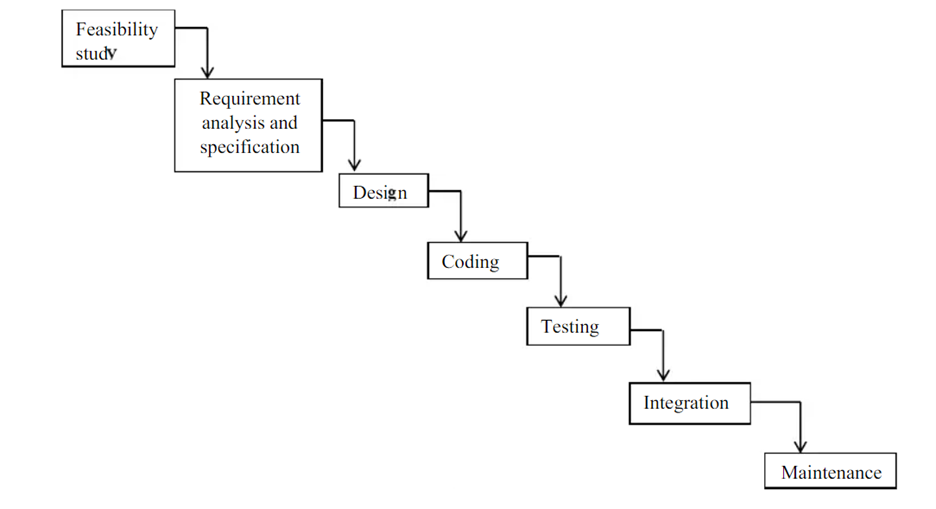
\includegraphics[width=10cm,height=6cm]{img/palnningmodel.png}
    \caption{Waterfall model}
    \label{fig:my_label}
\end{figure}
\newpage
\subsection{Justification for the methodology}
The waterfall methodology was worthwhile because this approach produced a complete quality system and error-free system due to the fact that every phase had to be completed before the next one began thus leaving no phase unattended. However, according to the data collected on the user requirements, there was a clear understanding of the user requirement hence no doubt on what was to be developed. Similarly, the approach was also less costly since there was no repeating of a process once completed and thus minimized wastage of resources as compared to other approaches such as the rapid prototyping methods.
\subsection{Research Methodology}
Research is a structured inquiry that utilizes acceptable scientific methodology to solve problems and create new knowledge that is generally applicable. Scientific methods consist of systematic observation, classification, and interpretation of data. Basically, research is a process of collecting, analyzing, and interpreting information to answer questions. Simply, a research methodology is a process of gaining information to gain and gather information about any specific project or topic which should be controller, rigorous, valid & verifiable, empirical, and finally critically evaluated. In this specific project about online air ticket management systems, several types of research have been done on the topics and tasks. The methods of research were:
\begin{itemize}
    \item 	Primary research:
\item Action Research
\item Quantitative Research
\item Secondary Research:
\item Survey
\item Research Qualitative
\item Experiment
\end{itemize}

The first stage of research methodology was section research and quantitative research methodology was followed. E-Ticket plays an important role in finding project requirements, system requirements and analytical methods. There are also lists of resources and guidelines to follow in e-ticket research to help with the project. On the other hand, the purpose of quantitative research is to employ mathematical models of phenomena, and the measurement method provides the central relationship of quantitative research.
Secondary research will be included, the case study project plan helps to find the basic idea of a case study project to find out the current in-depth situation and helps to critically evaluate the idea. On the other hand, qualitative research and experiments are holistic approaches to research methods. All of the above will help me find the research methodology and best comprehensive theory as well as system concepts for my project.
\newpage
\subsection{Context Mapping}
\begin{figure}[h]
    \centering
    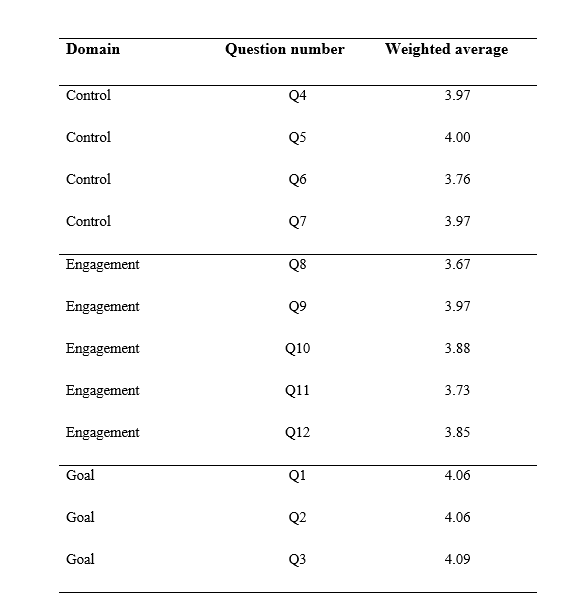
\includegraphics[height=10cm]{img/domainqu.png}

    \label{fig:my_label}
\end{figure}
\begin{figure}[h]
    \centering
    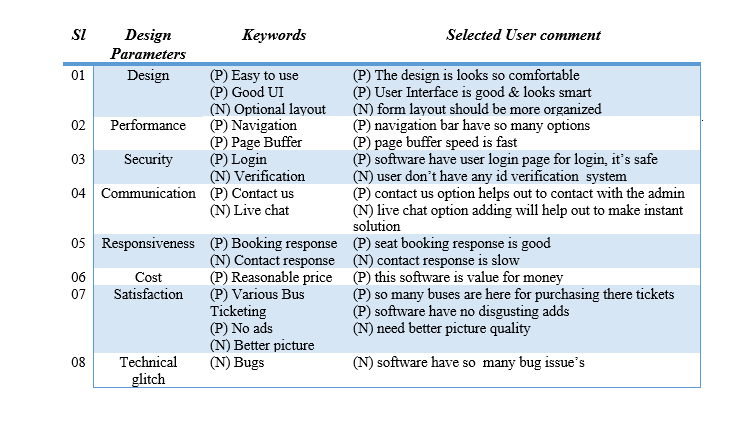
\includegraphics[width=10cm,height=6cm]{img/commet.png}
    \label{fig:my_label}
\end{figure}
\newpage
\begin{figure}[h]
    \centering
    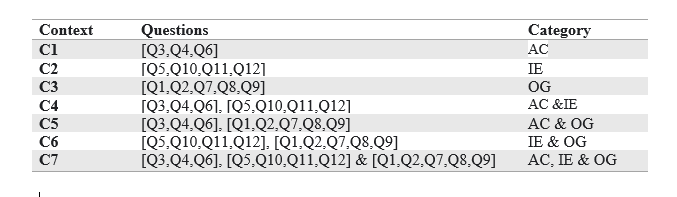
\includegraphics[width=10cm,height=6cm]{img/tabl1.png}
    \label{fig:my_label}
\end{figure}
\newpage
\begin{figure}[h]
    \centering
   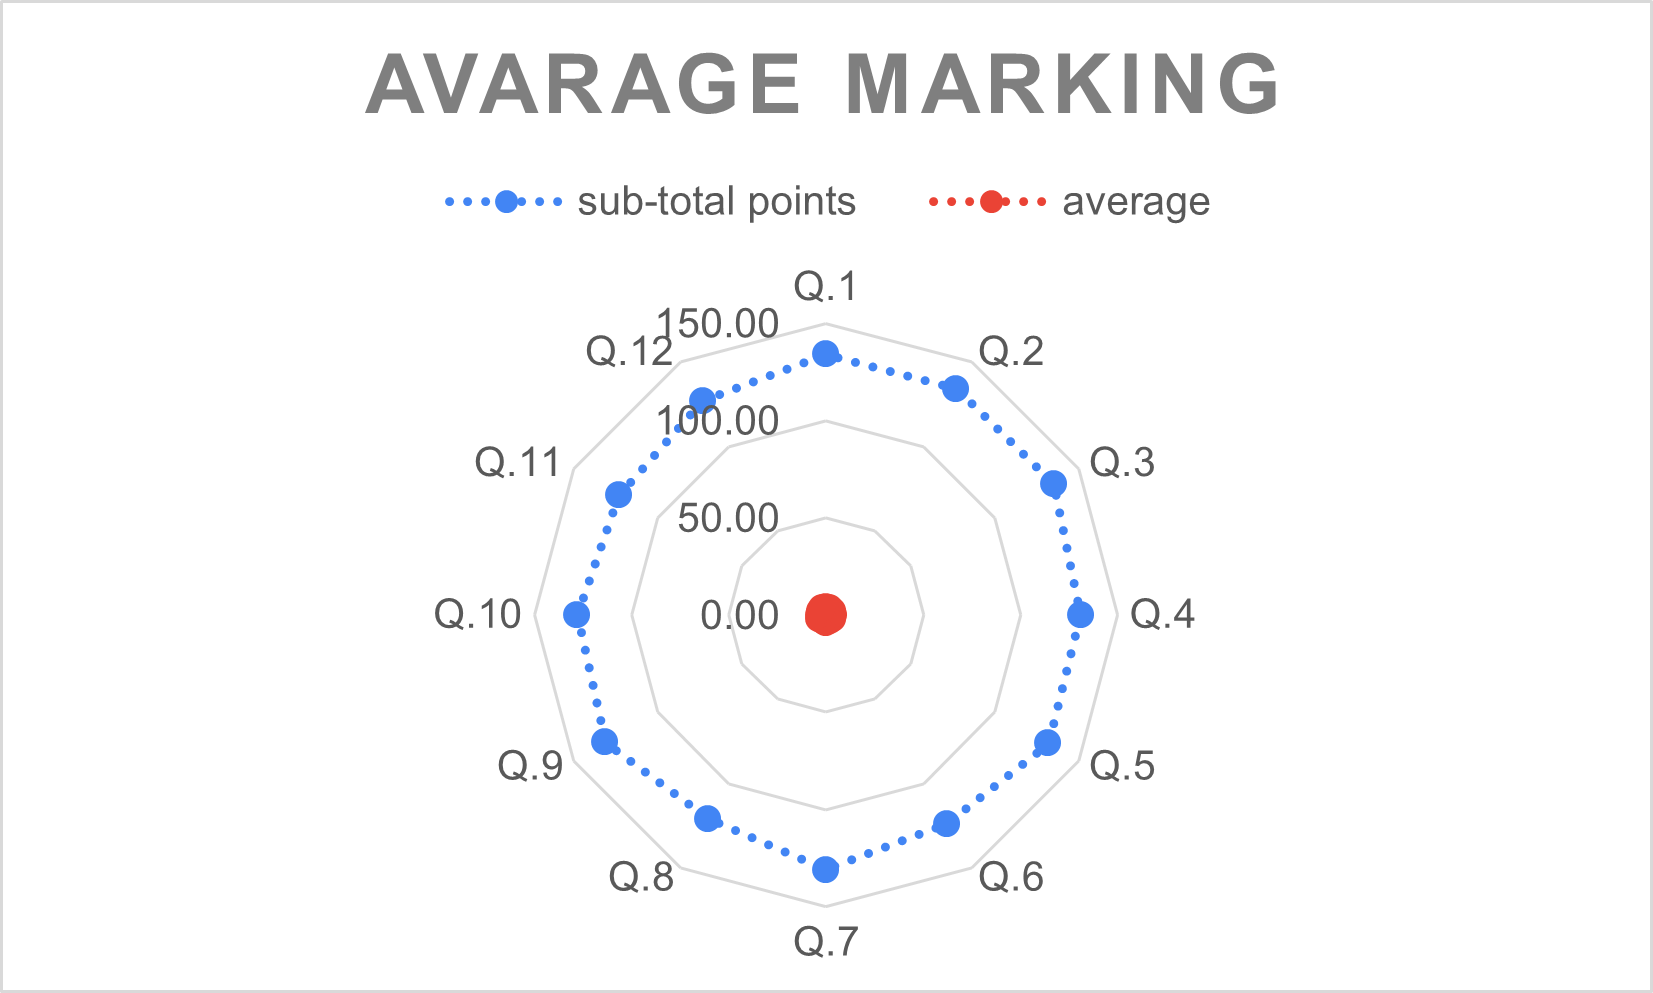
\includegraphics[width=10cm,height=8cm]{img/avaragemarking.png}
    \caption{Averaging Radar graph}
    \label{fig:my_label}
\end{figure}
\newpage
\begin{center}
    \section \huge \textbf{Chapter 04}
\end{center}
\subsection{Implementation}
As a result of this research, the model for e-ticketing buses, the implementation of some activities, the existence of activities, actions or processes of a system, a planned activity, and structure. To explain the proposed system, diagrams are used. A use case diagram is a diagram that represents interactions between use cases and actors.
\subsection{Context level diagram}
A data flow diagram (DFD) is a graphical representation of the "flow" of data through an information system, modeling aspects of its processes. A DFD shows what data will be input and output from the system, where the data will come from and where it will go, and where the data will be stored. Each process in the lower-level diagram of DFD can be broken down into more detailed DFDs at the next level. Top-level diagrams are often called context diagrams. It consists of a single process bit, which plays an important role in studying the current system.
\begin{figure}[h]
    \centering
    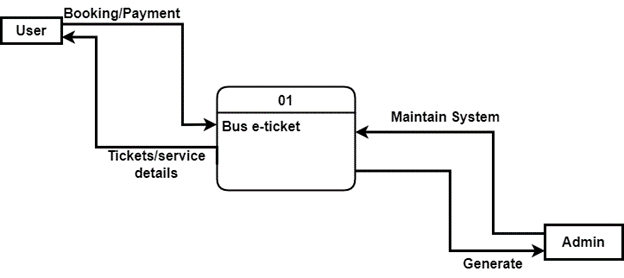
\includegraphics[width=10cm, height=6cm]{img/context.png}
    \caption{Context View of Online Bus Ticket Reservation System}
    \label{fig:my_label}
\end{figure}
\newpage
\subsection{Use case Diagram for Users and admin}
A use case is a methodology used in system analysis to identify, clarify and organize system requirements. The use case is made up of a set of possible sequences of interactions between systems and users in a particular environment and related to a particular goal. The method creates a document that describes all the steps taken by a user to complete an activity.
\begin{figure}[h]
    \centering
    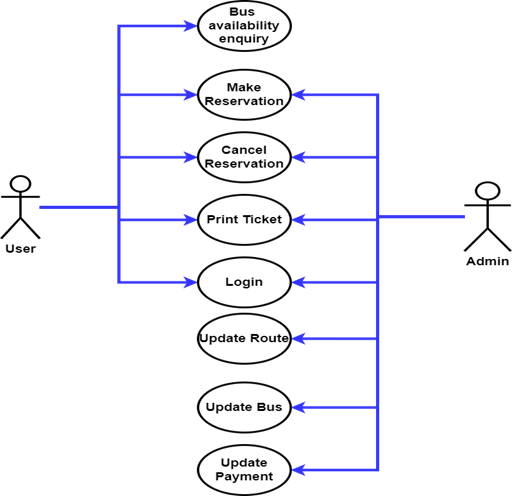
\includegraphics[width=10cm, height=6cm]{img/usecase.png}
    \caption{Use case Diagram}
    \label{fig:my_label}
\end{figure}
\newpage
\newpage
\begin{center}
    \section \huge \textbf{Web site Page Screenshot}
\end{center}
\subsection{Home page}
\begin{figure}[h]
    \centering
    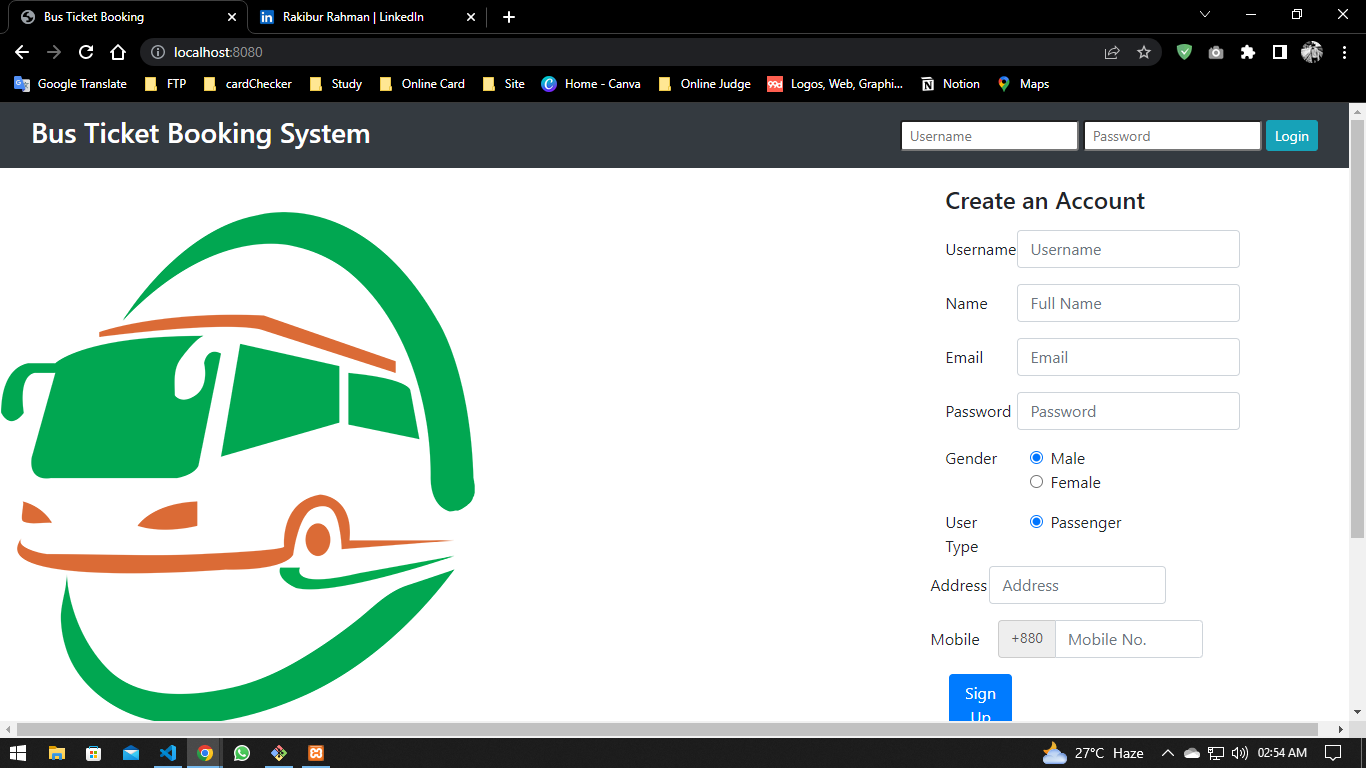
\includegraphics[width=10cm,height=8cm]{img/homepage.png}
    \caption{Home Page}
    \label{fig:my_label}
\end{figure}
\begin{figure}[h]
    \centering
    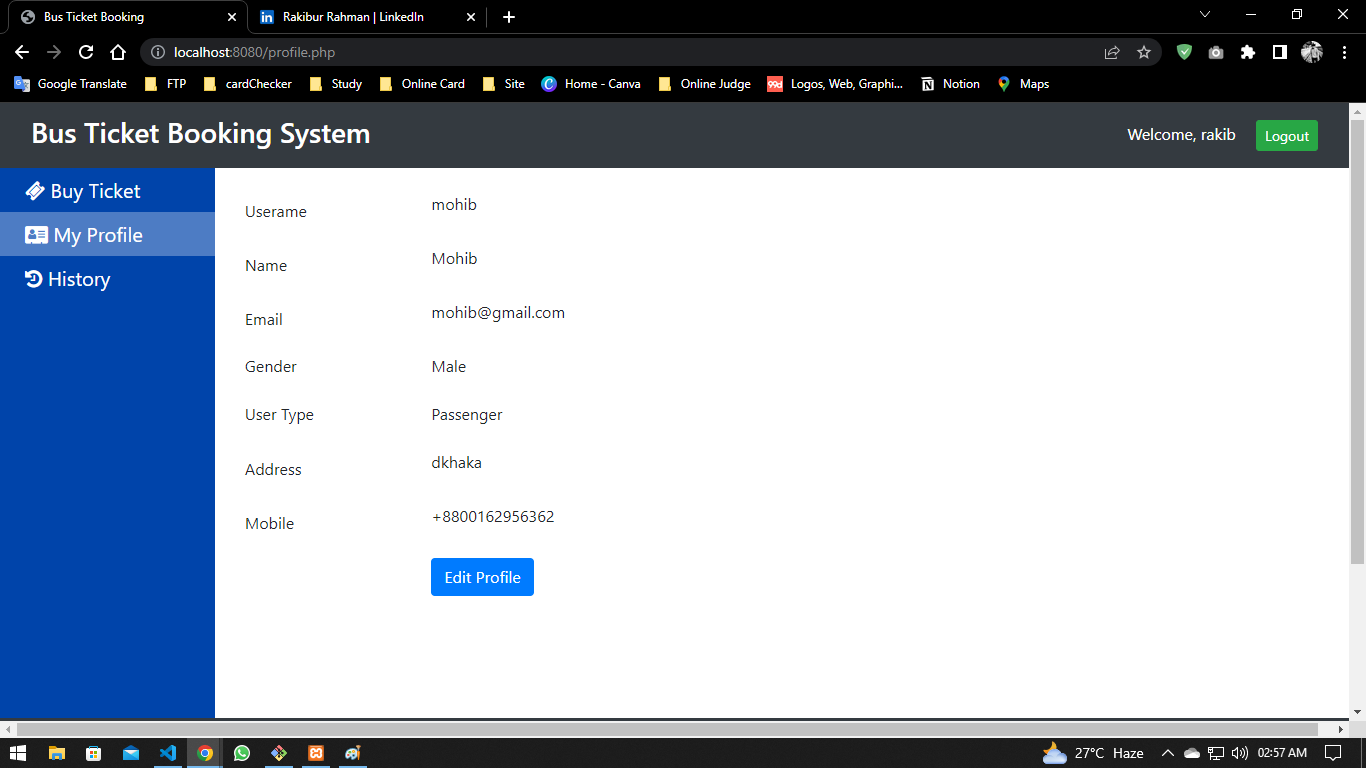
\includegraphics[width=10cm,height=8cm]{img/customer profile.png}
    \caption{Customer Profile}
    \label{fig:my_label}
\end{figure}
\begin{figure}[h]
    \centering
    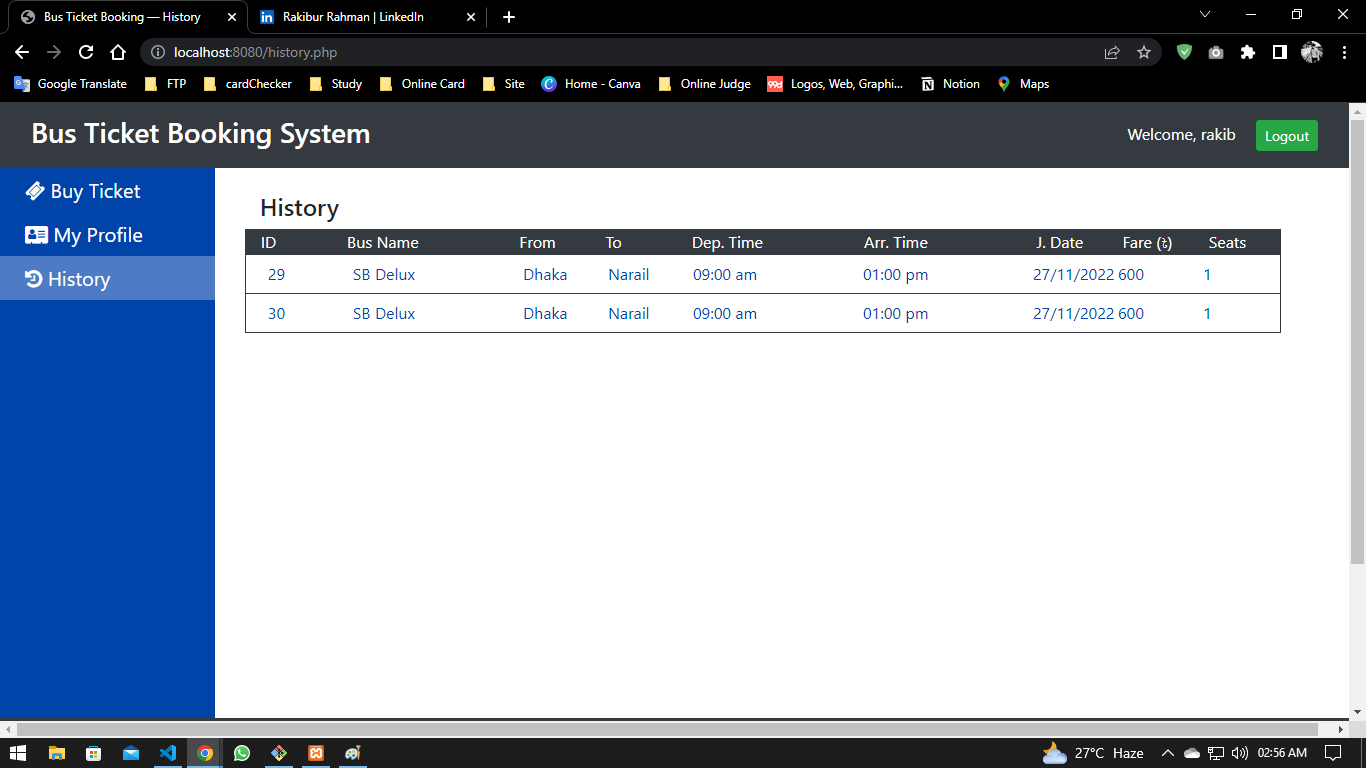
\includegraphics[width=10cm,height=8cm]{img/customer history.png}
    \caption{Customer History}
    \label{fig:my_label}
\end{figure}
\begin{figure}[h]
    \centering
    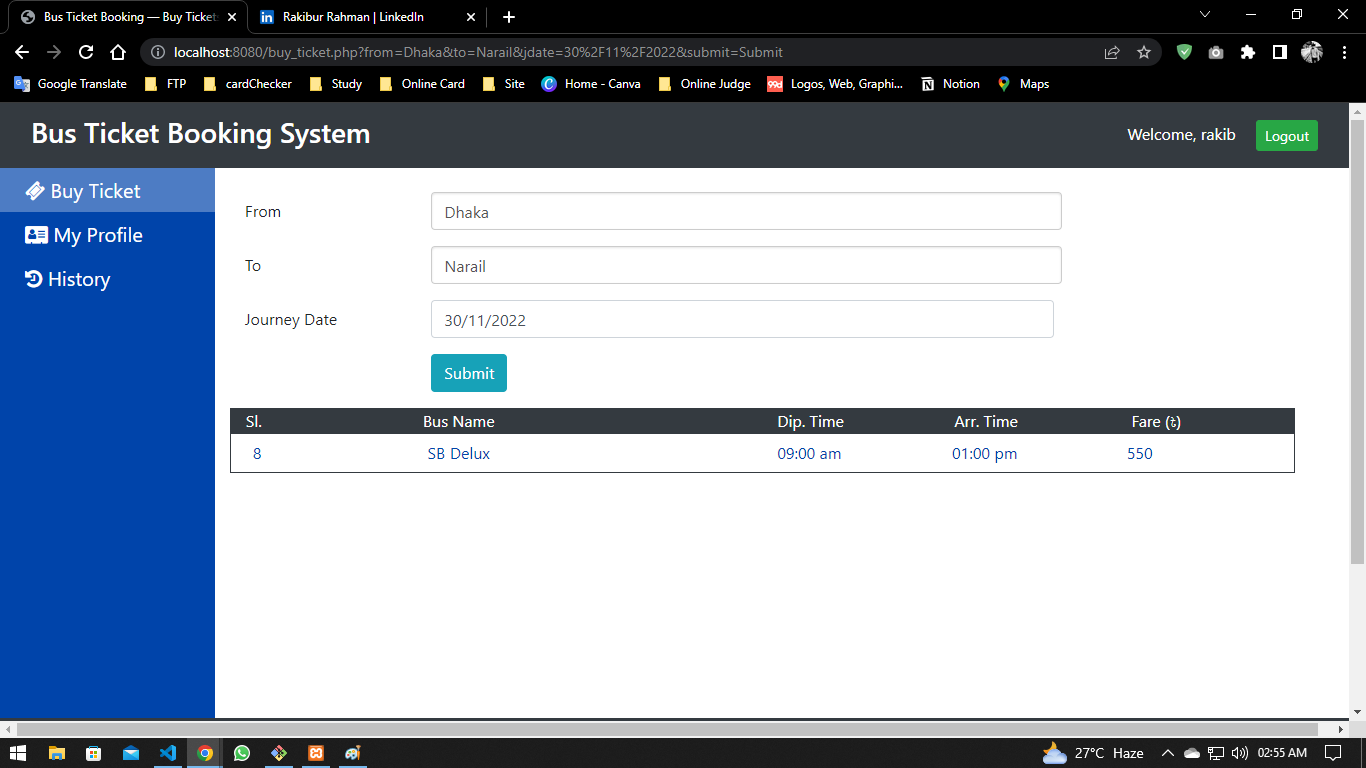
\includegraphics[width=10cm,height=8cm]{img/bussearch.png}
    \caption{Bus Search}
    \label{fig:my_label}
\end{figure}
\begin{figure}[h]
    \centering
    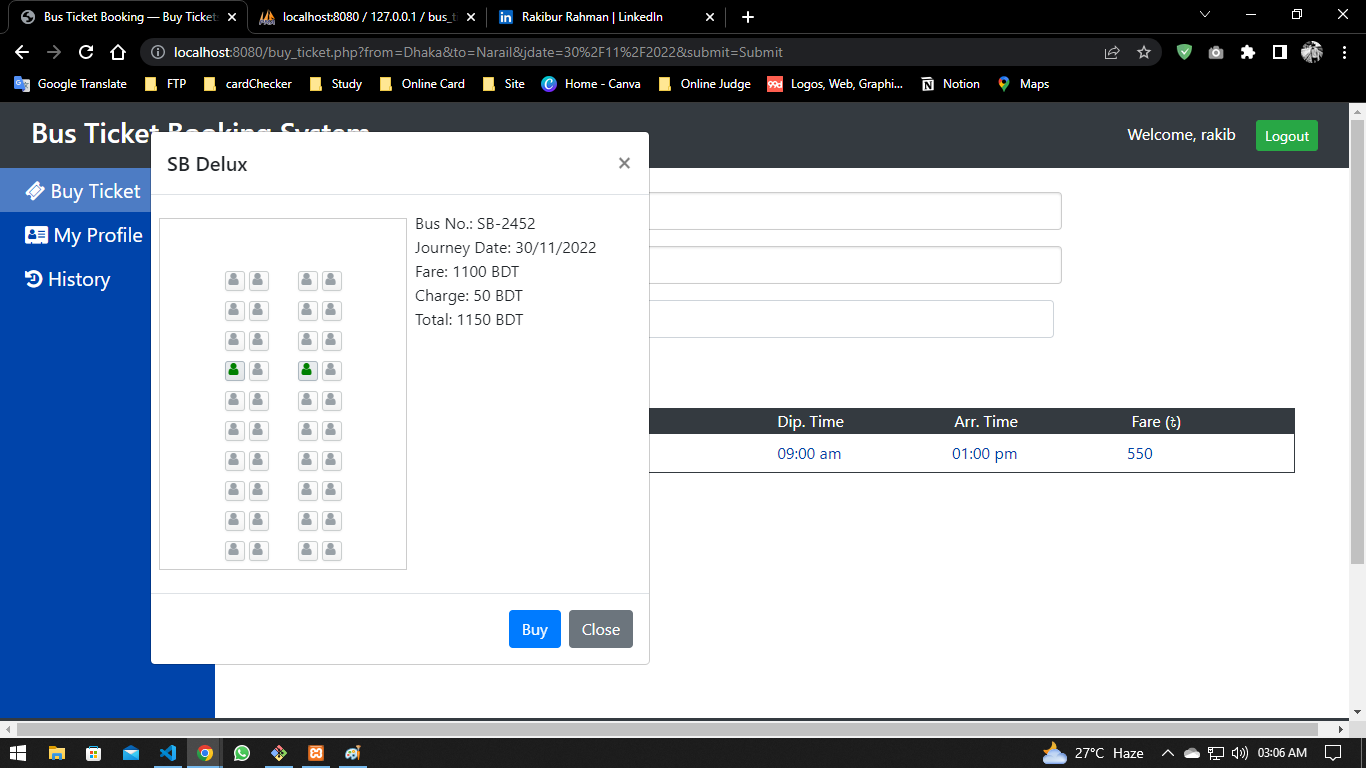
\includegraphics[width=10cm,height=8cm]{img/purchase ticket.png}
    \caption{Choose seat}
    \label{fig:my_label}
\end{figure}
\newpage
\begin{figure}[h]
    \centering
    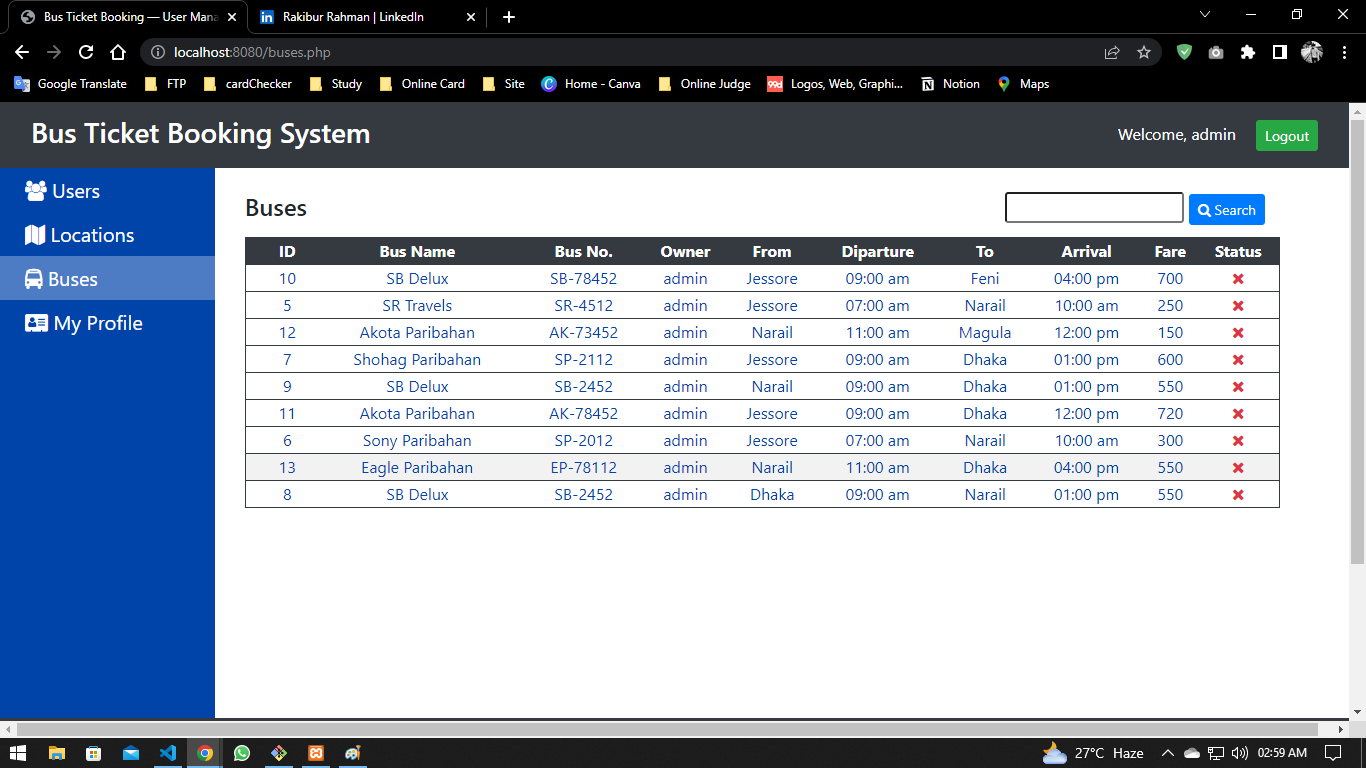
\includegraphics[width=10cm,height=8cm]{img/admin view bus.png}
    \caption{Admin View bus}
    \label{fig:my_label}
\end{figure}
\begin{figure}[h]
    \centering
  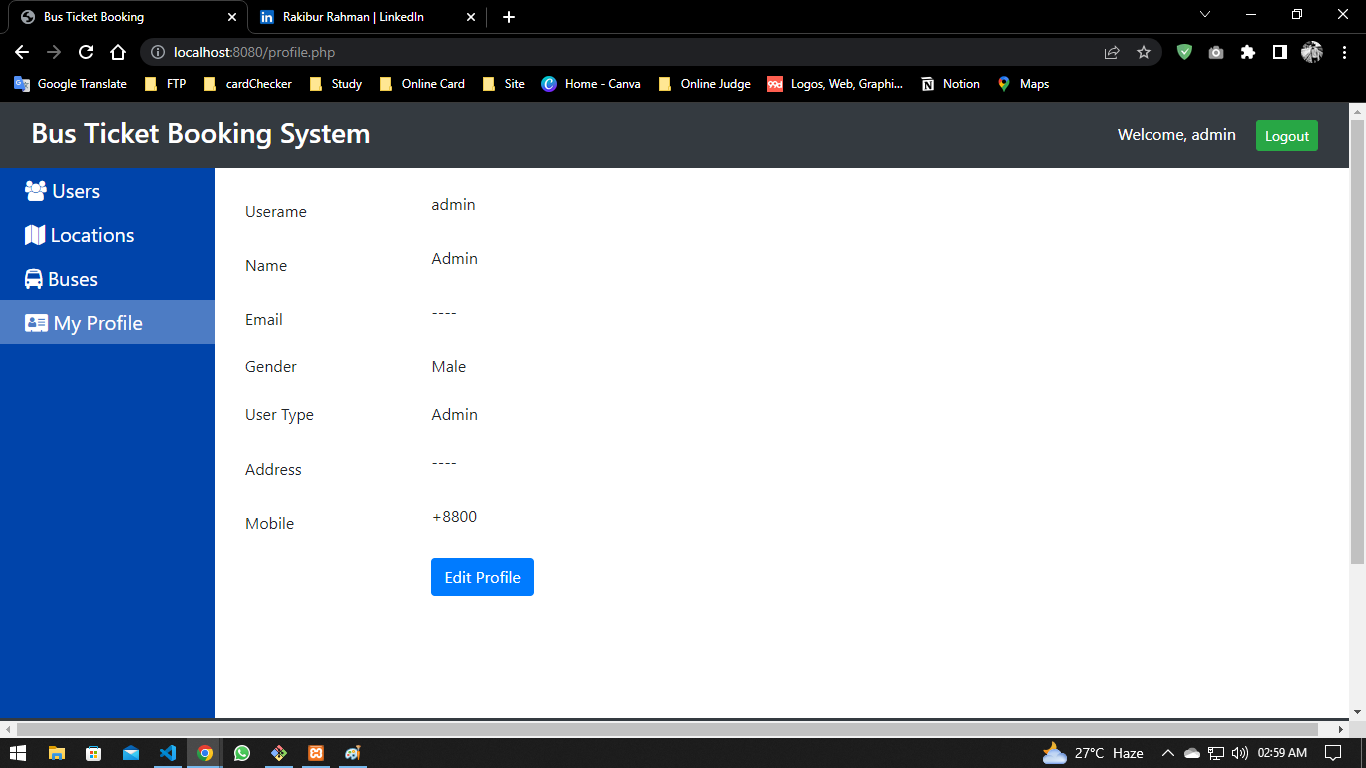
\includegraphics[width=10cm,height=8cm]{img/admin profile view.png}
    \caption{Admin Profile}
    \label{fig:my_label}
\end{figure}
\newpage
\begin{figure}[h]
    \centering
    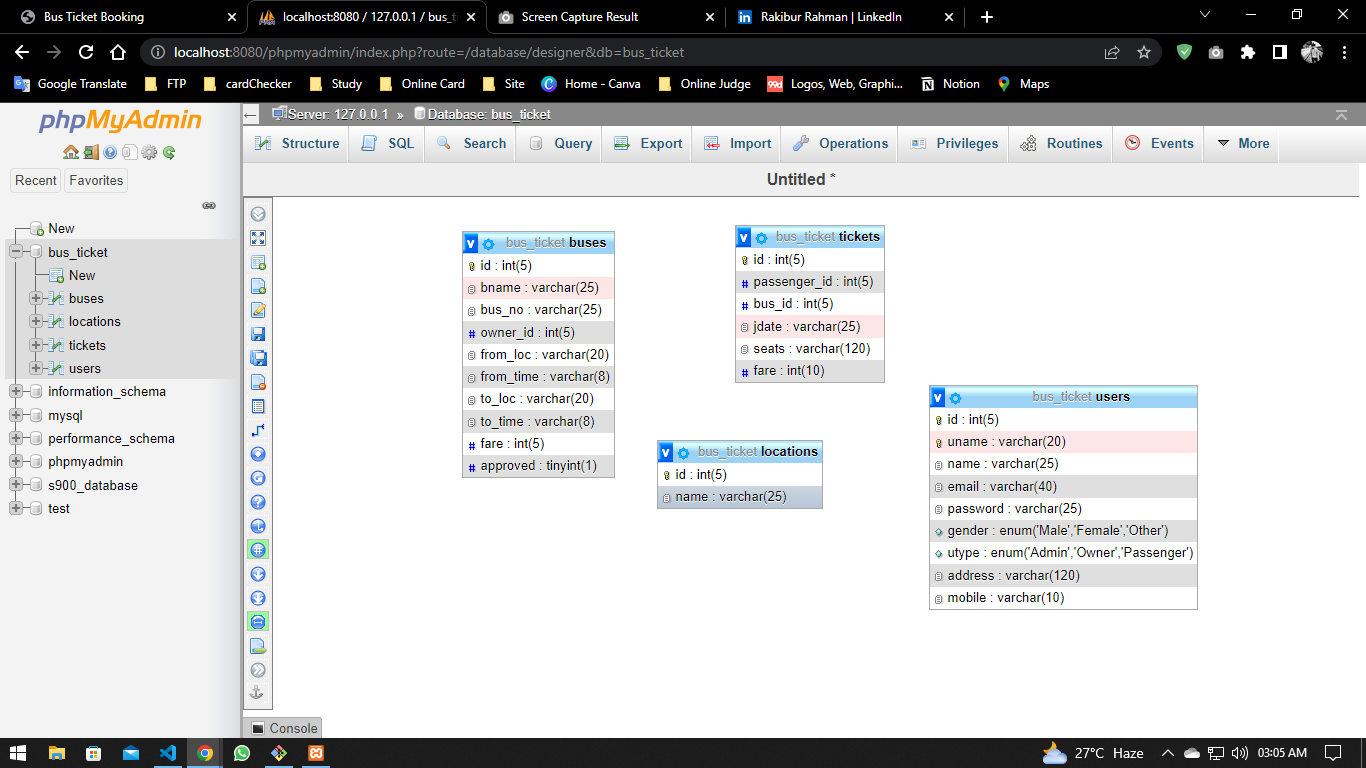
\includegraphics[width=10cm,height=8cm]{img/database.png}
    \caption{Database}
    \label{fig:my_label}
\end{figure}
\newpage
\begin{center}
 \huge \textbf{Chapter 05}
\end{center}
\section{Conclusion}[b]
Above all, it is clear that modern technology is taking place of everything where possible. It is saving our time and giving us the best benefit of the new era. The above project work is something that can bring up a revolutionary change in online ticket booking systems in my home country Bangladesh. The project is containing in-depth concept and system build-up for online air ticket management. This system will allow mass users in Bangladesh to book their air tickets online, which is easy, secure, and convenient. Whether there are numerous added benefits of this system that will help people in Bangladesh to travel comfortably. Though lacking software knowledge and information resources might be a problem for this website but future improvement works. Finally, I honestly hope this project work is just one step for Bangladesh and will bring something new to online users.
\newpage
\newpage








\end{document}
